\documentclass[a4paper, 12pt]{article}

\usepackage{ucs}
\usepackage[utf8x]{inputenc}
\usepackage[T1]{fontenc}
\usepackage[french]{babel}

\usepackage{microtype}

\usepackage{lmodern}
\usepackage[bitstream-charter]{mathdesign}

\usepackage[margin=1.5cm]{geometry}

\usepackage{color}
\definecolor{blue}{rgb}{0.38,0.58,0.81}
\definecolor{green}{rgb}{0.47,0.72,0.33}
\definecolor{red}{rgb}{0.91,0.34,0.32}
\definecolor{frame}{rgb}{0.70,0.70,0.70}
\definecolor{grey}{rgb}{0.97,0.97,0.97}

\PrerenderUnicode{é}

\usepackage{hyperref}
\hypersetup{
  pdftitle={Visualisation de données},
  pdfsubject={Devoir de programmation OpenGL - FlowVR},
  pdfauthor={Damien Gombault - Cyril Lavedrine},
  colorlinks,
  citecolor=black,
  filecolor=black,
  linkcolor=black,
  urlcolor=blue
}

\usepackage[pdftex]{graphicx}
\usepackage{keystroke}

\begin{document}

\thispagestyle{empty}

\begin{center}
\vspace*{\fill}

\hrule
\vspace{1cm}
{\Huge \textbf{Visualisation de données} \\}
{\LARGE Devoir de programmation OpenGL -- FlowVR \\}
\vspace{1cm}
\hrule

\vspace{2cm}

\includegraphics[width=5cm]{include/logos/universite.png}
\vspace{2cm}

{\Large
\textbf{Étudiants} \\
Damien GOMBAULT \\
Cyril LAVEDRINE \\
}

\vspace{4cm}

\large{1\ier{} avril 2009\\}

\vspace*{\fill}
\end{center}

\newpage

\renewcommand{\contentsname}{Sommaire}
\setcounter{tocdepth}{4}
\tableofcontents
\newpage

\section{Description de l'archive}

Voici une description du contenu de l'archive :

\begin{itemize}
\item \texttt{data/} : ce répertoire contient des exemples de terrain (grilles
de hauteurs, textures, et sources d'inondation)
\item \texttt{doc/} : ce répertoire contient ce rapport et ses sources au format
{\fontfamily{lmodern}\LaTeX}
\item \texttt{doxygen/} : ce répertoire contient la documentation du projet au
format Doxygen
\item \texttt{include/} : ce répertoire contient les \textit{headers}
nécessaires à la compilation du projet
\item \texttt{src/} : ce répertoire contient les sources C++ du projet
\item \texttt{tools/} : ce répertoire contient un outil en Python permettant de
découper les grilles de hauteurs
\item \texttt{make-clean.sh} : script shell permettant de nettoyer les sources
du projet
\item \texttt{make-doxygen.sh} : script shell permettant de générer la
documentation Doxygen
\item \texttt{make-simulation.sh} : script shell permettant de compiler le
projet
\item \texttt{simulation.csv} : fichier de configuration du réseau
FlowVR
\end{itemize}

\section{Installation}

\subsection{Dépendances}

Avant de pouvoir compiler le projet, vous devez d'abord installer \textbf{Qt} et
\textbf{FlowVR Suite} (ainsi que leurs dépendances). \\

Le projet a été testé uniquement sur \textbf{Debian squeeze/sid} avec les
versions suivantes des logiciels :

\begin{itemize}
\item FlowVR Suite \textbf{1.5}
\item Qt \textbf{4.5} (avec les modules \textbf{QtCore}, \textbf{QtGui} et
\textbf{QtOpenGL})
\item cmake \textbf{2.6}
\end{itemize}

\subsection{Compilation}

Le projet s'installe de la même façon que les autres applications FlowVR. Le
script shell \linebreak \texttt{make-simulation.sh} situé à la racine permet de
compiler le projet.

\subsection{Remarques}

N'oubliez pas de configurer les variables d'environnement nécessaires au bon
fonctionnement de FlowVR et du projet. Pour cela, il faut charger les scripts
\texttt{flowvr-config.sh} (fourni avec FlowVR) et \texttt{simulation-config.sh}
(créé pendant la compilation du projet) dans votre environnement en modifiant
par exemple les fichiers \texttt{\textasciitilde/.bashrc} et
\texttt{\textasciitilde/.bash\_profile}. \\

Si vous souhaitez faire fonctionner le projet en réseau, il est conseillé
d'utiliser les mêmes noms d'utilisateur et d'installer le projet dans la même
arborescence sur toutes les machines. \\

Pensez également à générer les clefs SSH, vérifier les connexions, autoriser
l'accès distant à X (commande \texttt{xhost +}), vérifier les noms des
machines (fichier \texttt{/etc/hosts}) et à configurer l'application (fichier
\texttt{simulation.csv}). \\

Pour de plus amples informations sur le fonctionnement et la configuration de
FlowVR, référez vous à son manuel d'utilisation\footnote{Manuel d'utilisation
de FlowVR \newline
\url{http://www-id.imag.fr/FLOWVR/manual/flowvr/flowvr-manual.pdf}}.

\section{Utilisation}

\subsection{Lancement}

Le projet se lance de la même façon que les autres applications FlowVR. Lancez
tout d'abord le démon \texttt{flowvrd} puis lancez la simulation avec la
commande \texttt{flowvr -x -l simulation}. \\

Une fenêtre de visualisation du terrain et de l'inondation devrait s'ouvrir :

\begin{center}
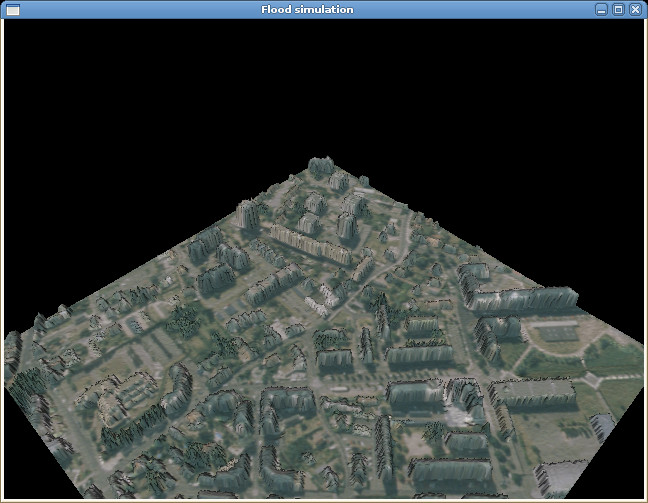
\includegraphics[width=0.75\textwidth]{include/captures/1.jpg}
\end{center}

Par défaut, une grille de taille $512\times512$ est chargée. Si votre carte
graphique n'est pas assez puissante (principalement au niveau de la quantité de
mémoire\footnote{Une carte graphique possédant 256 Mio de mémoire dédiée est
requise pour une grille de taille $512\times512$.}), vous pouvez choisir une
grille plus petite. Pour cela, vous devez modifier les fichiers
\texttt{include/simulation/components/metamoduleflood.comp.h} et
\texttt{include/simulation/components/metamoduleviewer.comp.h} et remplacer les
fichiers passées en paramètres aux modules dans \texttt{CmdLine}. Relancez
ensuite la compilation du projet.

\subsection{Contrôle de la caméra}

Vous pouvez déplacer la caméra en utilisant la souris et le clavier :

\begin{itemize}
\item clic gauche enfoncé ou \UArrow \DArrow \LArrow \RArrow : tourne la caméra
sur elle même
\item molette vers le haut ou \PgUp : déplace la caméra vers le haut
\item molette vers le bas ou \PgDown : déplace la caméra vers le bas
\item \keystroke{Z} : déplace la caméra vers l'avant
\item \keystroke{S} : déplace la caméra vers l'arrière
\item \keystroke{Q} : déplace la caméra vers la gauche
\item \keystroke{D} : déplace la caméra vers la droite
\item \Shift : accélère le déplacement de la caméra \\
\end{itemize}

\pagebreak

Voici une capture d'écran de la simulation après quelques secondes d'écoulement
de l'inondation et déplacement de la caméra :

\begin{center}
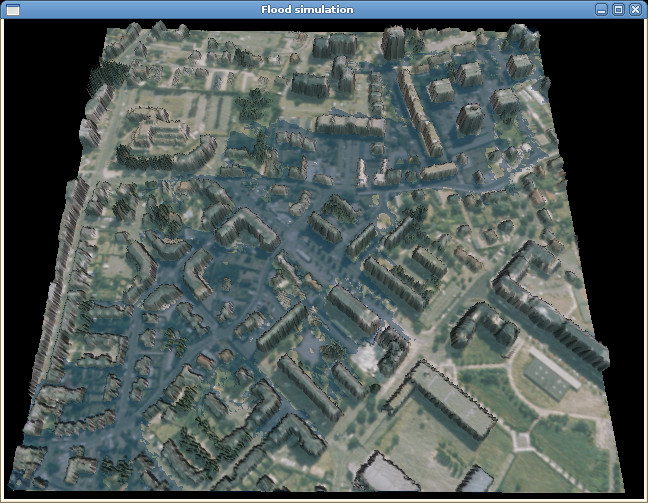
\includegraphics[width=0.75\textwidth]{include/captures/2.jpg}
\end{center}

\section{Implémentation}

\subsection{Description}

Le projet est composé de deux modules FlowVR. Le premier, nommé \texttt{viewer},
permet la visualisation du terrain et de l'inondation dans une scène OpenGL. Le
second, nommé \texttt{flood}, permet de calculer l'écoulement de l'inondation.

\subsubsection{Module \texttt{viewer}}

Ce module de visualisation est divisé en plusieurs classes. Voici leurs
descriptions.

\paragraph{Classe \texttt{Camera}}

Cette classe implémente le déplacement de la caméra dans la scène OpenGL. Il
s'agit d'une caméra de type vol libre.

\paragraph{Classe \texttt{DTM}}

Cette classe implémente le terrain. Elle permet de charger le terrain à partir
d'un fichier \texttt{grd} et initialise ensuite les différentes structures de
données nécessaires (sommets, index, normales et coordonnées de textures) pour
l'affichage du terrain à l'écran. Pour obtenir de bonnes performances, cette
classe utilise des \textit{vertex buffer objects} statiques pour stocker les
données directement dans la mémoire vidéo.

\paragraph{Classe \texttt{FlowVR}}

Cette classe permet l'initialisation des ports de ce module pour les
communications FlowVR. Deux ports sont ainsi créés : \texttt{dtmOut} pour
l'envoi du terrain au module d'inondation et \texttt{waterIn} pour la réception
des données de l'inondation.

\paragraph{Classe \texttt{FlowVRThread}}

Les communications de ce module sont déléguées à un \textit{thread}. Cette
classe permet ainsi l'envoi du terrain au module d'inondation et la réception
des données de l'inondation. L'utilisation d'un \textit{thread} dédié aux
communications permet d'éviter de figer l'interface graphique quand le module
est en attente d'un message.

\paragraph{Classe \texttt{Light}}

Cette classe implémente la gestion de la lumière de la scène OpenGL.


\paragraph{Classe \texttt{OpenGLScene}}

Il s'agit de la classe principale de ce module. Elle implémente l'interface
graphique et gère les événements du clavier et de la souris. Cette classe
initialise également les autres éléments de ce module.

\paragraph{Classe \texttt{Point3d}}

Cette classe implémente un point dans l'espace. Elle permet d'effectuer diverses
opérations (addition, multiplication, \dots).

\paragraph{Classe \texttt{Water}}

Cette classe implémente l'eau. À l'instar de la classe \texttt{DTM}, elle
s'occupe d'initialiser les structures nécessaires à l'affichage de l'eau à
l'écran. Pour obtenir de bonnes performances, cette classe utilise des
\textit{vertex buffer objects} dynamiques. Lorsque cette classe reçoit un signal
\texttt{updated()} de la classe \texttt{FlowVRThread}, elle met à jour les VBO
avec les nouvelles valeurs reçues par le module d'inondation.

\subsubsection{Module \texttt{flood}}

Ce module dédié au calcul de l'écoulement de l'inondation est divisé en
plusieurs classes. Voici leurs descriptions.

\paragraph{Classe \texttt{Flood}}

Cette classe implémente l'écoulement de l'inondation. Elle permet de charger les
sources de l'inondation à partir d'un fichier \texttt{water}. L'écoulement est
ensuite mis à jour à intervalles réguliers, tous les $\frac{1}{10}$ seconde. Une
fois le calcul terminé, le niveau d'eau des cases où il y a une source est
augmenté.  Puis un message contenant les nouvelles valeurs est envoyé au module
de visualisation. La méthode d'écoulement implémentée est similaire à celle
présentée dans l'énoncé du devoir.

\paragraph{Classe \texttt{FlowVR}}

Cette classe permet l'initialisation des ports de ce module pour les
communications FlowVR. Deux ports sont ainsi créés : \texttt{waterOut} pour
l'envoi des données de l'inondation au module de visualisation et \texttt{dtmIn}
pour la réception du terrain.

\subsubsection{Connexions entre modules}

Les modules sont reliés par deux connexions synchrones. \\

La première connexion relie le port de sortie \texttt{dtmOut} du module de
visualisation au port d'entrée \texttt{dtmIn} du module d'inondation. Cette
connexion est utilisée une seule fois, lors de l'initialisation du module
d'inondation, afin de recevoir les données du terrain. \\

La seconde connexion relie le port de sortie \texttt{waterOut} du module
d'inondation au port d'entrée \texttt{waterIn} du module de visualisation.
Cette connexion est utilisée à chaque itération de mise à jour de l'écoulement
de l'inondation.

\pagebreak

\subsection{Déroulement de la simulation}

Voici le déroulement du fonctionnement de l'application.

\paragraph*{Étape n\up{o}1}

\begin{center}
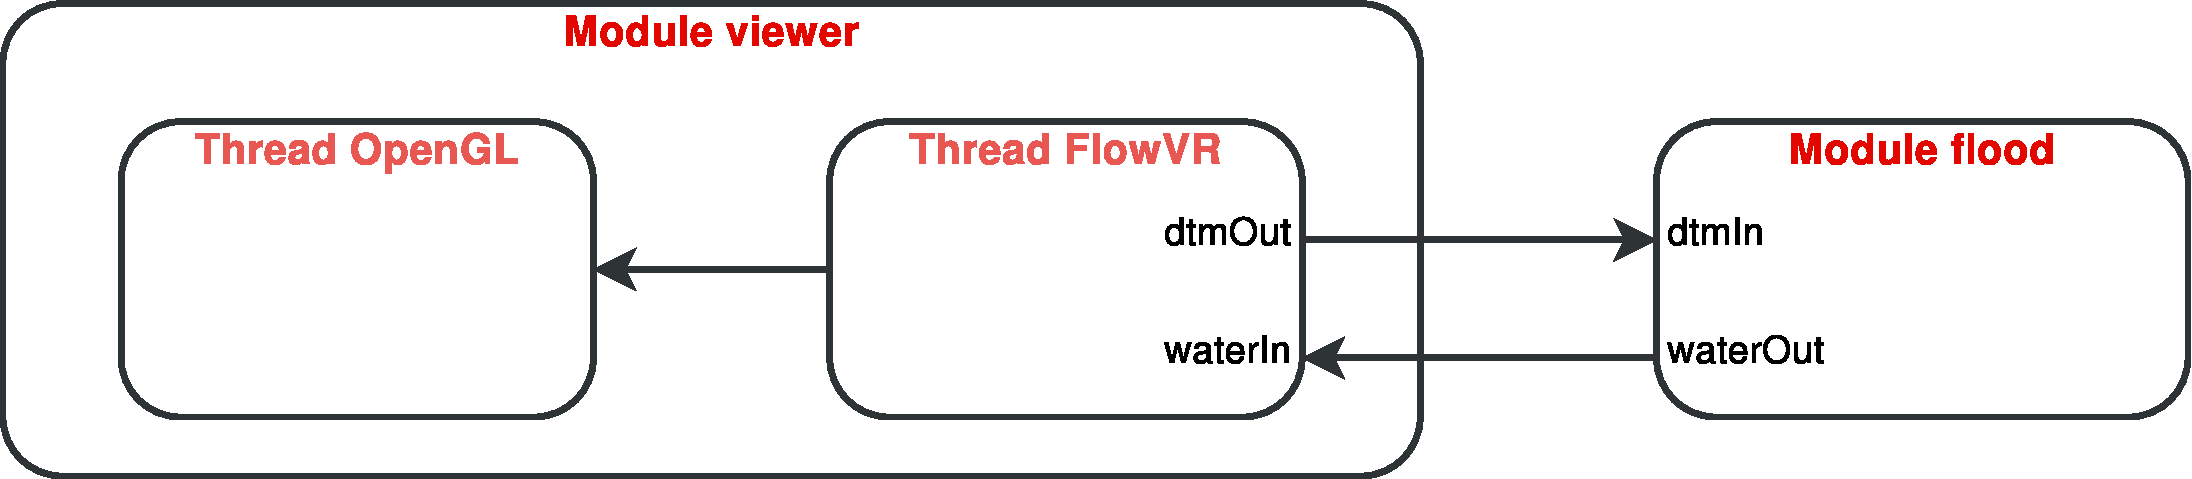
\includegraphics[scale=0.4]{include/schemas/1.pdf}
\end{center}

Les deux modules FlowVR se lancent et les ports de communication sont
initialisés.

\paragraph*{Étape n\up{o}2}

\begin{center}
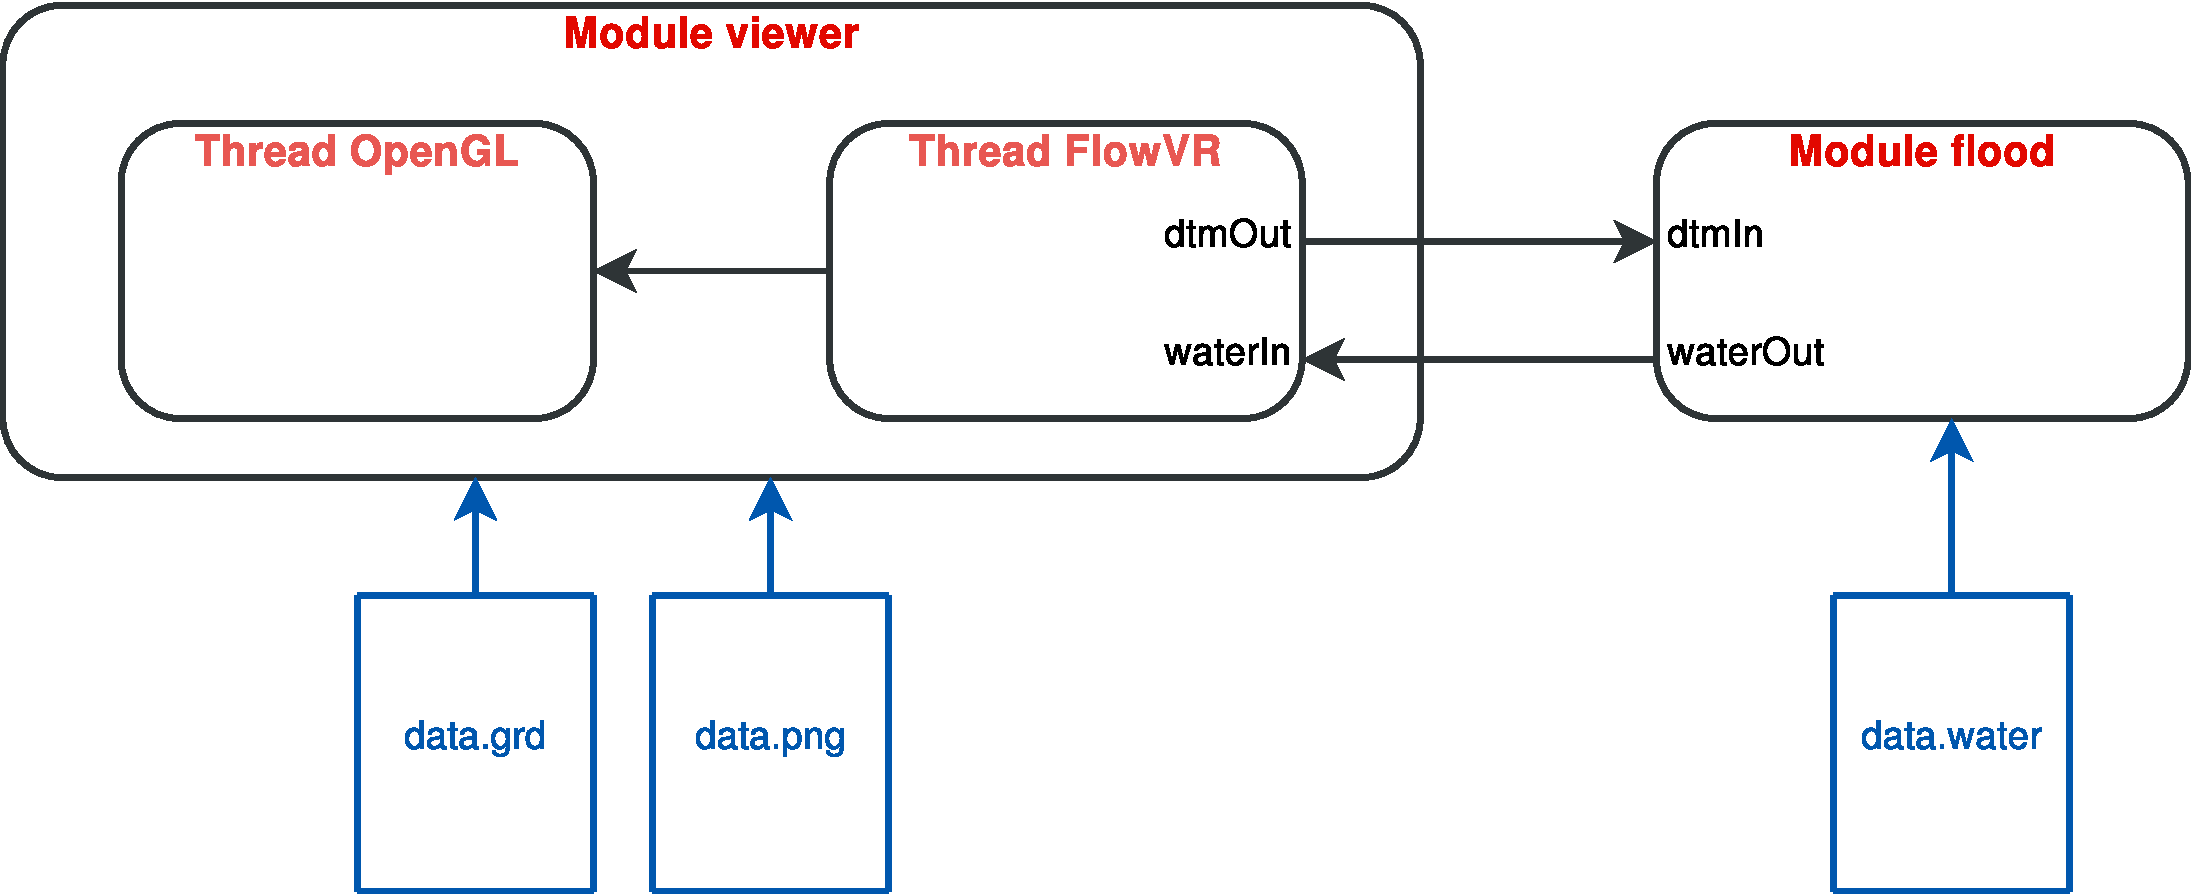
\includegraphics[scale=0.4]{include/schemas/2.pdf}
\end{center}

Le module de visualisation charge le terrain à partir du fichier \texttt{grd}
contenant les hauteurs. Il charge également la texture à partir du fichier
\texttt{png}. Le module d'inondation charge les sources de l'inondation à
partir du fichier \texttt{water}.

\paragraph*{Étape n\up{o}3}

\begin{center}
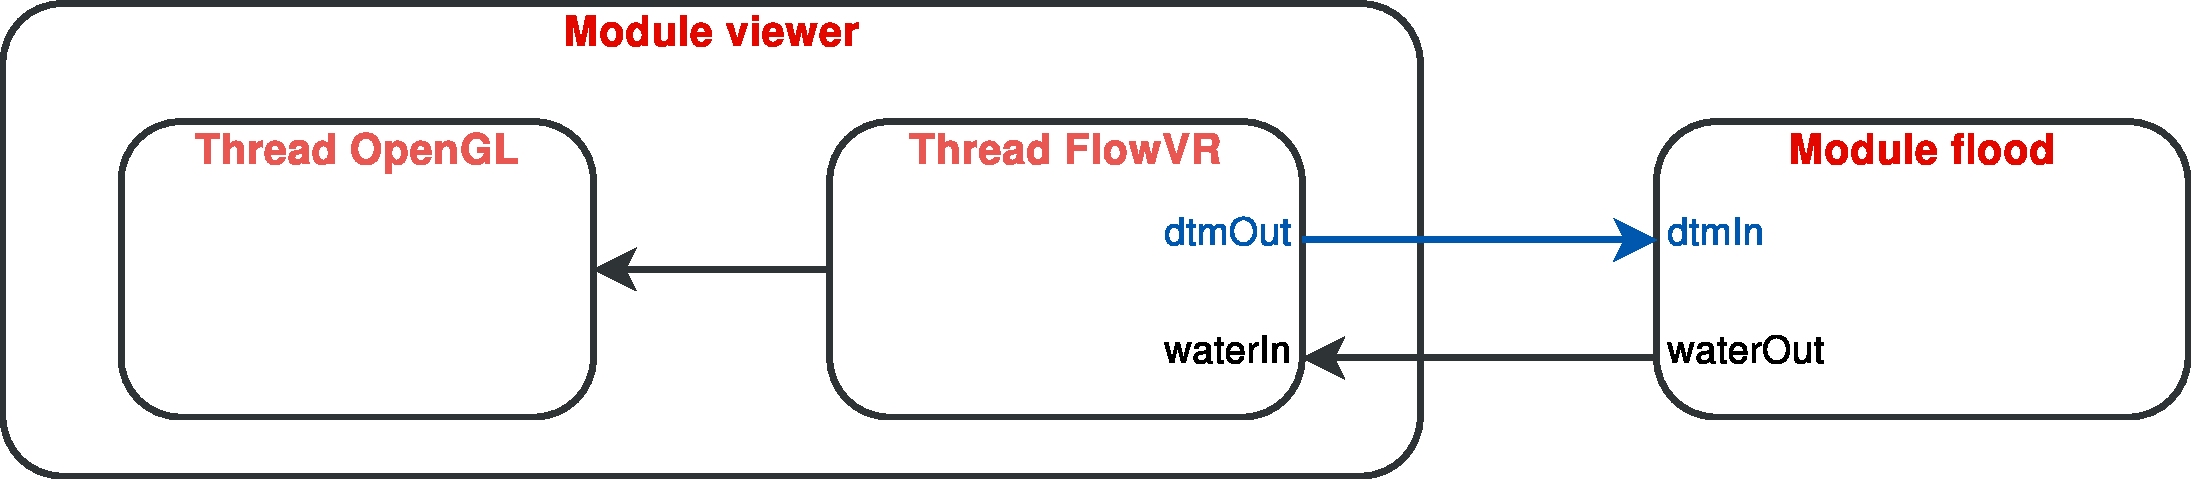
\includegraphics[scale=0.4]{include/schemas/3.pdf}
\end{center}

Le module de visualisation envoie les données du terrain au module d'inondation.
Le nombre de lignes et de colonnes du terrain sont d'abord envoyées. Ensuite,
les hauteurs sont transmises sous la forme d'un tableau de flottants. Les
données sortent du port \texttt{dtmOut} du module de visualisation et entrent
par le port \texttt{dtmIn} du module d'inondation.

\pagebreak

\paragraph*{Étape n\up{o}4}

\begin{center}
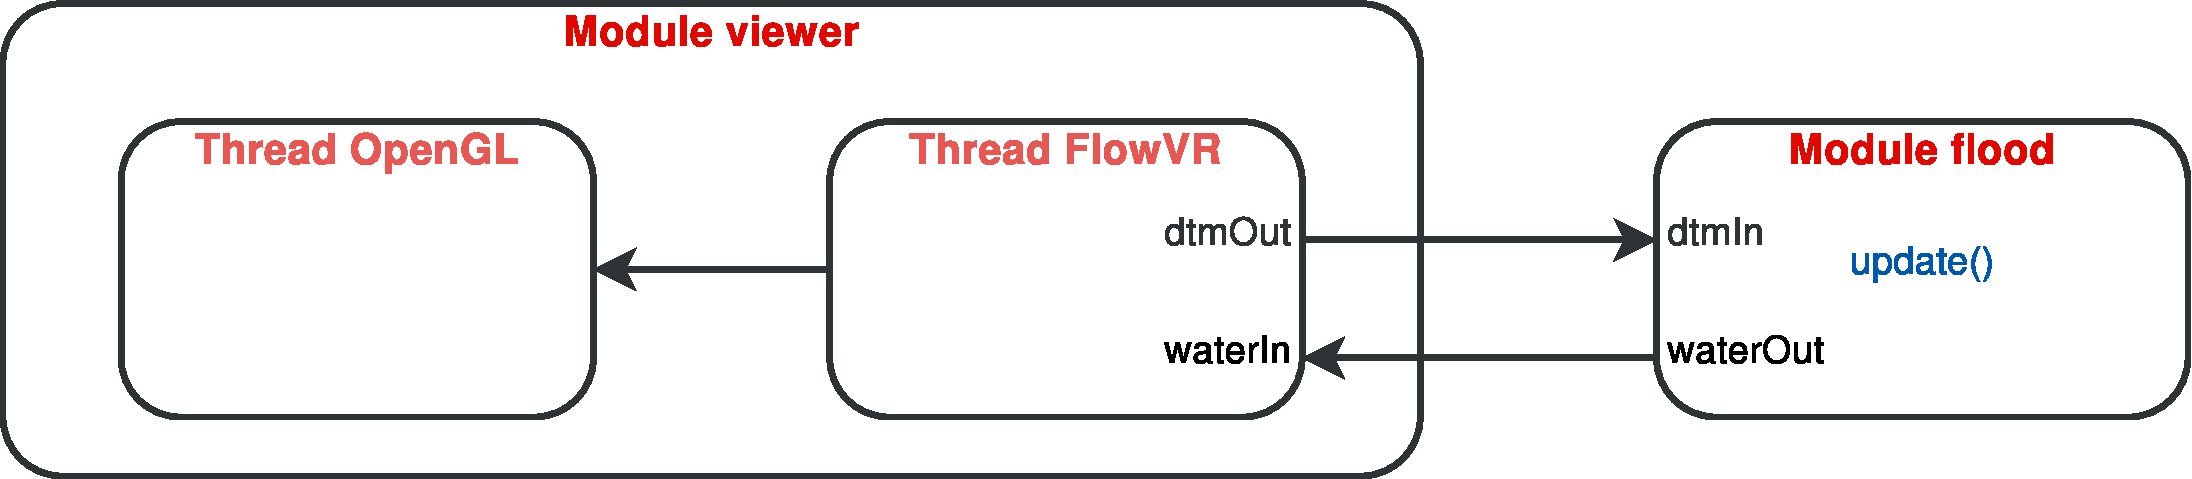
\includegraphics[scale=0.4]{include/schemas/4.pdf}
\end{center}

Le module d'inondation possède toutes les informations nécessaires pour
commencer à calculer les niveaux de l'eau. Il effectue donc une itération de
mise à jour des niveaux.

\paragraph*{Étape n\up{o}5}

\begin{center}
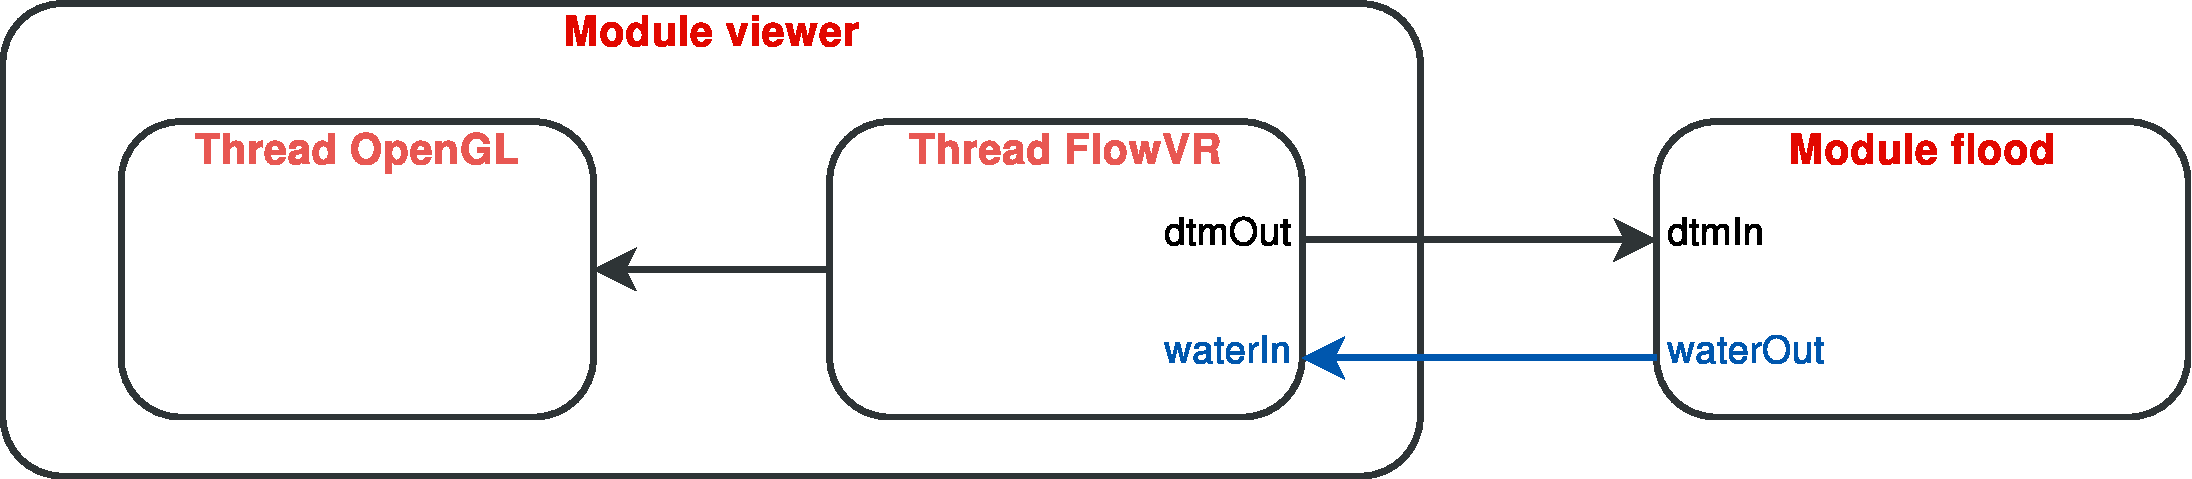
\includegraphics[scale=0.4]{include/schemas/5.pdf}
\end{center}

Une fois les nouveaux niveaux calculés, il envoie les nouvelles valeurs au
module de visualisation. Les données sortent du port \texttt{waterOut} du module
d'inondation et entrent par le port \texttt{waterIn} du module de visualisation.
Les données sont envoyées sous la forme d'un tableau de flottants.

\paragraph*{Étape n\up{o}6}

\begin{center}
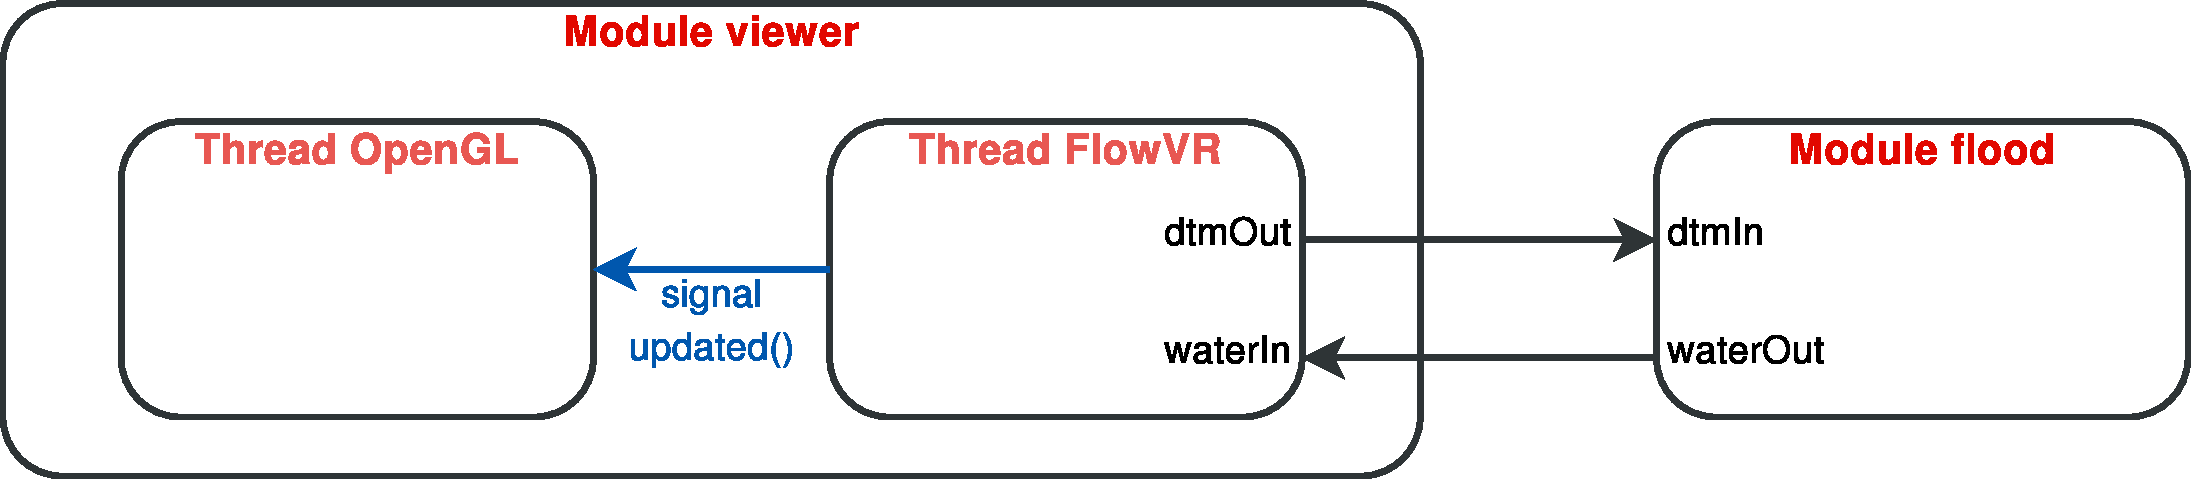
\includegraphics[scale=0.4]{include/schemas/6.pdf}
\end{center}

Une fois toutes les données des niveaux reçues, le \textit{thread} chargé des
communications FlowVR envoie un signal au \textit{thread} principal,
chargé de l'affichage, pour lui indiquer que les données ont été mises à jour.

\paragraph*{Étape n\up{o}7}
\begin{center}
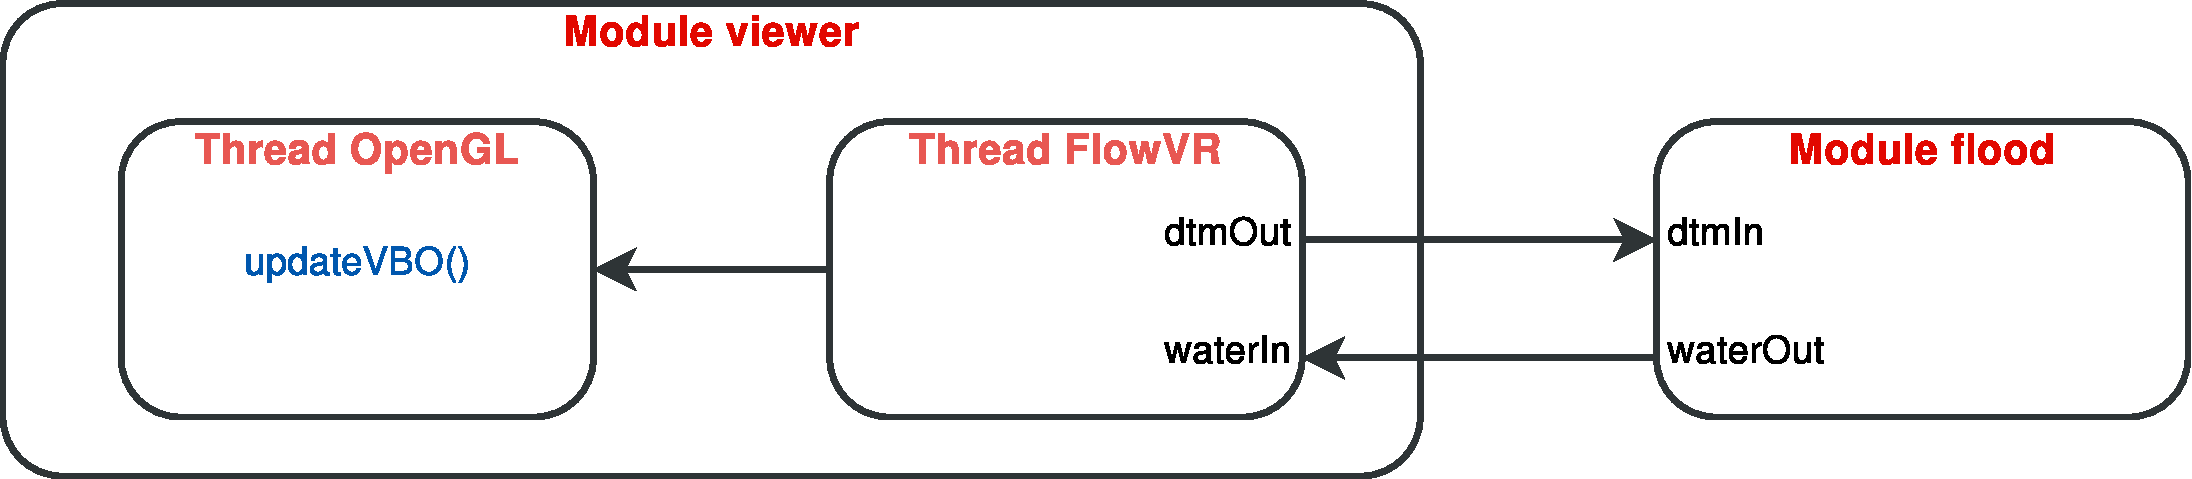
\includegraphics[scale=0.4]{include/schemas/7.pdf}
\end{center}

Le \textit{thread} principal chargé de l'affichage peut ensuite mettre à jour
les \textit{vertex buffer objects} pour l'affichage de l'eau. \\

On recommence ensuite à partir de l'étape n\up{o}4. Pendant toutes ces étapes,
le module de visualisation affiche de façon totalement indépendante le terrain
et l'eau et ne se préoccupe ainsi pas de l'inondation. Ceci permet d'avoir un
affichage fluide de la simulation.

\end{document}
